\subsection{Arbitrary Lagrangian Eulerian}
\begin{frame}{Problem}

\begin{block}{}
Solve a FLuid/Structure interaction (FSI) :
\end{block}


\begin{block}{Problem :}

\begin{itemize}
\item Lagrangian approach can not consider all fluid particles.

\item Eulerian approach can not be used because the boundaries are moving.

\item FEM : the mesh must move with the structure but re-mesh at each time step is too expensive.
\end{itemize}
\end{block}
\end{frame}

%****************************************************************************

\begin{frame}{ALE}

\begin{block}{Idea : }
Use Arbitrary Lagrangian Eulerian method :

$\rightarrow$ Solve equation with adapted formulation.
\end{block}

\begin{itemize}
\item Lagrangian approach is considered for structure,

\item Eulerian approach is used for fluid,

\item Move the mesh smoothly with the boundaries.
\end{itemize}
\end{frame}

%****************************************************************************

\begin{frame}{}

\begin{block}{}
$\rightarrow$ ALE map :

$\mathcal{A}^t : \left\{ 
\begin{array}{rcl}
\widehat{\Omega} & \longrightarrow  & \Omega(t)\\
\widehat{\mathbf{x}} & \longmapsto & \mathbf{x} ( \widehat{\mathbf{x}} , t)
\end{array}
\right.$
\end{block}

\begin{figure}[H]
\begin{center}
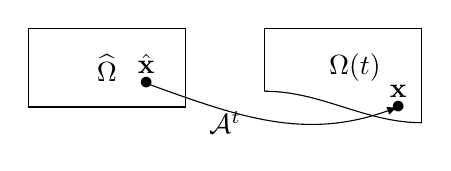
\begin{tikzpicture}[scale=1]
\draw (0,0) -- (2,0) -- (2,1) -- (0,1) -- (0,0);
\draw (1,0.5) node{$\widehat{\Omega}$} ;
\draw (1.5,0.3) node[above]{$\hat{\mathbf{x}}$} ;
\draw (1.5,0.3) node {$\bullet$} ;
\draw (3,1) -- (5,1);
\draw [domain=0:2] plot (\x+3,{(0.2*sin((0.5*pi*(\x+1)) r))}) ;
\draw [domain=0:1] plot (5,{(0.2*sin((0.5*pi*3) r)-1)*\x+1}) ;
\draw [domain=0:1] plot (3,{(0.2*sin((0.5*pi) r)-1)*\x+1}) ;
\draw (4.15,0.5) node{$\Omega(t)$} ;
\draw (4.7,0) node[above]{$\mathbf{x}$} ;
\draw (4.7,0) node {$\bullet$} ;
\draw[->,>=latex] (1.5,0.3) to[out=-20,in=-160] (4.7,0);
\draw (2.5,-0.2) node{$\mathcal{A}^t$} ;
\end{tikzpicture}
\end{center}
\end{figure}

\begin{columns}
\column{0.45\textwidth}

\begin{block}{Reference domain (Lagrangian)}
Square $\widehat{\Omega} = \left[ 0,1 \right]^2$, boundaries :
\begin{itemize}
\item $\widehat{\Gamma}_{in} = \{ 0 \} \times \left[ 0,1 \right]$,

\item $\widehat{\Gamma}_{s} = \left[ 0,1 \right] \times \{ 1 \} $,

\item $\widehat{\Gamma}_{out} = \{ 1 \} \times \left[ 0,1 \right]$,

\item $\widehat{\Gamma}_{b} = \left[ 0,1 \right] \times \{ 0 \} = \widehat{\gamma}_b \times \{ 0 \}$.
\end{itemize}
\end{block}



\column{0.45\textwidth}

\begin{block}{Physical domain (Eulerian)}
$\Omega$ fluid domain, boundaries :
\begin{itemize}
\item $\Gamma_{in} = \{ 0 \} \times \left[ b_z(0,t),1 \right]$,

\item $\Gamma_{s} = \left[ 0,1 \right] \times \{ 1 \} $,

\item $\Gamma_{out} = \{ 1 \} \times \left[ b_z(1,t),1 \right]$,

\item $\Gamma_{b} = \left[ 0,1 \right] \times \{ b_z(x,t) \}$ with $x \in \left[ 0,1 \right]$
\end{itemize}
\end{block}

\end{columns}

\end{frame}

%*************************************************************************

\begin{frame}

Then 
$$\mathbf{x} = \mathcal{A}^t ( \widehat{\mathbf{x}} ) = \widehat{\mathbf{x}} + \underbrace{\widehat{\mathbf{d}_{\delta}} ( \widehat{\mathbf{x}}, t)}_{\text{displacement}} $$

where $\widehat{\mathbf{d}_{\delta}}$ is given by a PDE to be smooth.

\begin{block}{$\widehat{\Omega} \rightarrow \Omega(t)$}
If $\widehat{u} : \widehat{\Omega} \rightarrow \mathbb{R}^d$

Then $u = \widehat{u} \circ \left( \mathcal{A}^t \right)^{-1} : \Omega(t) \overset{\mathcal{A}^t}{\longrightarrow} \widehat{\Omega} \overset{\widehat{u}}{\longrightarrow} \mathbb{R}^d$

$$\widehat{u} ( \widehat{ \mathbf{x} } ) = u \left( \underbrace{\mathcal{A}^t ( \widehat{\mathbf{x}}}_{= \mathbf{x}} ), t \right)$$
\end{block}

\end{frame}


\begin{frame}

\begin{alertblock}{}
$\mathbf{x} \in \Omega(t)$ is time dependant!
\end{alertblock}

Then, defining the mesh velocity :

$$\mathbf{\widehat{w}}( \mathbf{\widehat{x}}, t) = \dfrac{\partial \mathcal{A}^t}{\partial t}(\mathbf{\widehat{x}}) = \dfrac{\partial \mathbf{\widehat{d}_{\delta}}}{\partial t}(\mathbf{\widehat{x}},t)$$

We have the following result :

\begin{block}{}
$$\dfrac{\mathcal{D}\mathbf{u}}{\mathcal{D}t} = \left.\frac{\partial \mathbf{u}}{\partial t}\right|_x + \mathbf{w}\cdot \nabla \mathbf{u}$$
\end{block}






\end{frame}








